% !TeX program = pdflatex
\documentclass[12pt,letterpaper]{article}
\usepackage[utf8x]{inputenc}
\usepackage{ucs}
\usepackage[spanish,mexico]{babel}
\usepackage{amsmath}
\usepackage{amsfonts}
\usepackage{amssymb}
\usepackage{makeidx}
\usepackage{xcolor}
\usepackage{graphicx}
\usepackage[useregional]{datetime2}
\usepackage{fancyhdr}
% % % %Geometry
\usepackage{geometry}%\usepackage[showframe]{geometry}
%\usepackage{layout}
\setlength{\voffset}{-0.7in}
\setlength{\headsep}{10pt}
\setlength{\textheight}{10.5in}
\usepackage{wasysym} %emoticons :)
\usepackage[oldstyle]{kpfonts}
%\usepackage[T1]{fontenc}
\newcommand{\fej}{\relax\hfill\ifmmode{\lower.5ex\hbox{{\textcolor{blue}{\LARGE\smiley al 15pt}}}}\else\lower.5ex\hbox{{\textcolor{blue}{\LARGE \smiley}}}}  % Smiley emoticon :)
\author{\textsc{Manuel López Mateos}}
% % % % % % % Para usar título, autor y fecha por separado.
\makeatletter
\let\newtitle\@title
\let\elautor\@author
\let\newdate\@date
\makeatother
%
%
% % % % Enviroments
\newenvironment{definition}[1][Definición.]{\begin{trivlist}
		\item[\hskip \labelsep {\bfseries #1}]}{\end{trivlist}}
% % % % % % % % % % % %
%
% % % % % % % % Headers
\pagestyle{fancy}
\fancyhf{}
\rhead{\color{olive}\hfill \DTMnow}
\lhead{\color{olive}\elautor}
\cfoot{\thepage}
\renewcommand{\headrule}{\color{olive}\hrule}
%\rfoot{}
% % % % % % %
%\title{Tangentes horizontales y verticales}
%\author{Manuel López Mateos}
\linespread{1.08}         % Palatino needs more leading (space between lines)
\begin{document} %\layout
\noindent Encuentra los puntos en que tiene tangente horizontal o vertical la gráfica de la función $y=(x-4)\sqrt[3]x$.

\medskip
La pendiente de una recta horizontal es $0$ y de una recta vertical, bueno, digamos que si una recta \emph{tiende} a ser vertical su \emph{pendiente tiende a infinito}.

\medskip
Así, nos piden hallar los puntos sobre la gráfica de la función donde la tangente tiene pendiente $0$ o \emph{infinito}. La derivada de la función da la pendiente de la tangente. La función es
\begin{align*}
y&=(x-4)\sqrt[3]x\\
&=(x-4)x^{1/3}\\
&=x^{4/3}-4x^{1/3}.
\end{align*}

La derivada es
\begin{align*}
y'&=\frac{4}{3}x^{1/3}-\frac{4}{3}x^{-2/3}\\
\noalign{\smallskip}
&=\frac{4}{3}x^{-2/3}(x-1)\\
&=\frac{4(x-1)}{3x^{2/3}}.
\end{align*}

El valor de la derivada es $0$ si el denominador es distinto de cero y el numerador es igual a cero, lo cual sucede si $x=1$. En la gráfica de la función, el punto $y$ correspondiente es $-3$. Así, en el punto de coordenadas $(1,-3)$ la gráfica de $y=(x-4)\sqrt[3]x$ tiene tangente horizontal, a saber la recta con ecuación $y=-3$.

De la fórmula de la derivada vemos que si $x$ tiende a cero, el numerador tiende a $-4$ y el denominador tiende a $0$ por lo que, cuando $x\to 0$, $y'\to \infty$. El punto $y$ correspondiente es $0$, luego en el punto de coordenadas $(0,0)$ de la gráfica, la función $y=(x-4)\sqrt[3]x$ tiene tangente vertical, a saber, la recta con ecuación $x=0$.

\begin{figure}[h]
\begin{center}
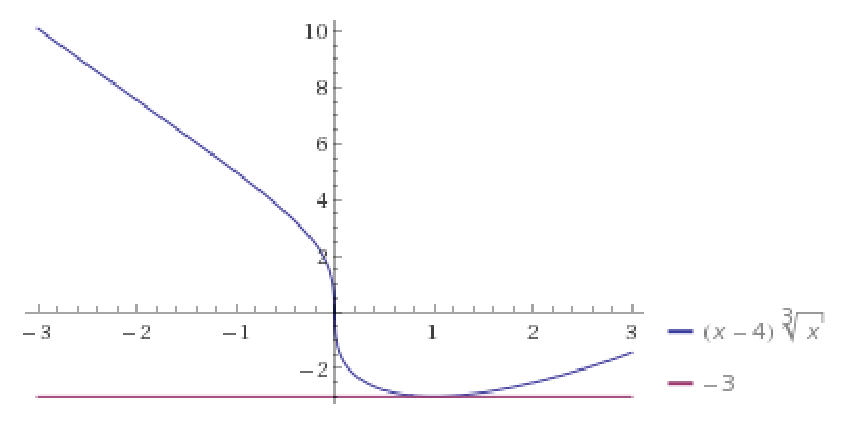
\includegraphics[scale=0.6]{img/6.fighorizontalesyverticales.pdf}
\caption{\small Tangente horizontal en $x=1$, tangente vertical en $x=0$.}
\end{center}
\end{figure}

\fej
\end{document}